\documentclass[12pt]{beamer}
\usepackage[utf8]{inputenc} % style d'écriture
\usepackage[T1]{fontenc}      % package
\usepackage[francais]{babel}  % package pour langue française
\usepackage{graphicx}
\usepackage{subcaption}
\usepackage{url}
\usepackage{color}
\usepackage{geometry}
\usepackage{amssymb}

% William PENSEC, étudiant en Master 2 LSE 2020/2021

\usetheme[secheader]{Madrid}
\beamertemplatenavigationsymbolsempty
\setbeamertemplate{frametitle continuation}{}

\title[Compte rendu de stage n\textsuperscript{o}6]{Coopération de drones dans un système hétérogène}
\subtitle{Compte rendu de stage n\textsuperscript{o}6}
\author{William \textsc{Pensec}}
%\author{William \textsc{Pensec}}
%\author{William \textsc{Pensec}}
\institute[Lab-STICC]{Lab-Sticc}
\date{26 mai 2021}

%\AtBeginSection[]
%{
%\begin{frame}<beamer>{Sommaire}
%\tableofcontents[currentsection,currentsubsection, 
%    hideothersubsections, 
%    sectionstyle=show/shaded,
%]
%\end{frame}
%}

\begin{document}
	% ---------------------------------------------------------------- %
	\begin{frame}
		\begin{titlepage}
			\begin{figure}[H]
				\centering
				
\includegraphics[scale=.15]{labsticc.png}
				\hspace{3cm}
				
\includegraphics[scale=.3]{ubo.png}
			\end{figure}
		\end{titlepage}
	\end{frame}
	
	% ---------------------------------------------------------------- %
	\section*{Sommaire}
	\begin{frame}
		\frametitle{Sommaire}
		\begin{center}
			\tableofcontents
		\end{center}
	\end{frame}
	%
	% ---------------------------------------------------------------- %
	\section{Positionnement du drone}	
	\begin{frame}[allowframebreaks]
    	\frametitle{Positionnement du drone}
    	    \begin{block}{}
				\begin{itemize}
    	        \setbeamertemplate{itemize items}[triangle]
				    \item Limite de 4 cartes
				    \item Les cartes supplémentaires ne sont pas prises en compte
				    \item Le drone prend l'ancre de référence et 3 autres ancres (normalement les plus proches)
				\end{itemize}
			\end{block}
			
			\begin{figure}[H]
				\centering
				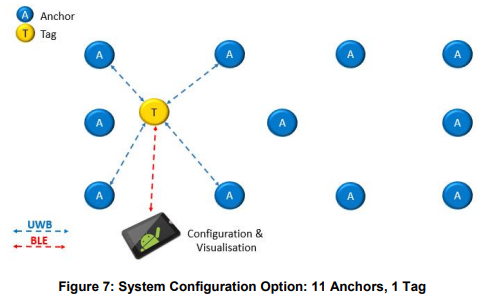
\includegraphics[scale=0.5]{ancres11.png}
			\end{figure}
	\end{frame}
	%
	% ---------------------------------------------------------------- %
	\section{Librairies pour le positionnement du drone}	
	\begin{frame}[allowframebreaks]
    	\frametitle{Librairies pour le positionnement du drone}
    	    \begin{block}{}
				\begin{itemize}
    	        \setbeamertemplate{itemize items}[triangle]
				    \item Bancroft : GPSTk\footnote{\url{https://github.com/SGL-UT/GPSTk}} $\rightarrow$ librairie Open Source fournie par l'Université du Texas à Austin (Space and Geophysics Laboratory (SGL))
				    \item Newton : Codes trouvés sur internet à tester
				\end{itemize}
			\end{block}
	\end{frame}
	%
	%% ---------------------------------------------------------------- %
	\section{A faire}
	\begin{frame}
	\frametitle{A faire}
	    \begin{alertblock}{}
    	    \begin{itemize}
    	    \setbeamertemplate{itemize items}[triangle]
    	        \item Finir de tester le code des méthodes Bancroft / Newton
    	        \item Parser la ligne lue pour enregistrer les valeurs avant lecture par une méthode de positionnement
    	    \end{itemize}
	    \end{alertblock}
	\end{frame}
	%
	%% ---------------------------------------------------------------- %/
\end{document}